\documentclass[12pt,a4paper,twoside,titlepage,openright]{book}
\usepackage[MeX]{polski}
\usepackage[utf8]{inputenc}
\usepackage{enumitem} % słownik pojęć
\usepackage{amsmath}
\usepackage{tabularx} % tabele
\usepackage[usenames,dvipsnames,svgnames,table]{xcolor} % kolory jak~się chce gdzieś użyć
\usepackage{graphicx} % żeby ryciny i~zdjęcia były
\usepackage{listings} % syntax highlighting
\usepackage{verbatimbox} % marginesy dla~tabel
\usepackage{emptypage} % usuwa nagłówki i~numery stron z~pustych stron
\usepackage{afterpage} % to zapobiega ustawianiu obrazka PO tym
\usepackage{filecontents} % pozwala na wstawienie bibliografi
\usepackage{setspace} % interlinia
\onehalfspacing
\graphicspath{{figures/}} %Setting the graphicspath
% PAGE LAYOUT
%\usepackage{showframe} % debug
\marginparwidth 0pt
\marginparsep 0pt
\usepackage[top=2.5cm,bottom=3cm,inner=4.5cm,outer=3cm]{geometry}

% HEADER, FOOTER
\usepackage{fancyhdr} 
\pagestyle{fancy}

%kropki w~spisie tresci
\makeatletter
\def\numberline#1{\hb@xt@\@tempdima{#1.\hfil}}
\makeatother

% CHAPTER TITLE

%kropki po~tytułach rodziałów
\makeatletter
\def\@makechapterhead#1{%
  \vspace*{50\p@}%
  {\parindent \z@ \raggedright \normalfont
	\ifnum \c@secnumdepth >\m@ne
	  \if@mainmatter
	   \huge\bfseries \@chapapp\space \thechapter.
	   \par\nobreak
	   \vskip 20\p@
	\fi
   \fi
   \interlinepenalty\@M
   \Huge \bfseries #1\par\nobreak
   \vskip 40\p@
  }}
\makeatother

% SPIS TREŚCI

%kropki w~spisie tresci
\makeatletter
\def\numberline#1{\hb@xt@\@tempdima{#1.\hfil}}
\makeatother

% TYTUŁY ROZDZIAŁÓW

%kropki po~tytułach rozdziałów
\makeatletter
\renewcommand*\@seccntformat[1]%
{\csname the#1\endcsname.\enspace}
\makeatother


% KONFIGURACJA WYGLĄDU NAGŁÓWKA TEGO CO SIĘ POWTARZA

\fancyhead{} 
\fancyhead[LE]{\rightmark}
\fancyhead[RO]{\leftmark}

% WYGLĄD TABEL

% vertical padding
\renewcommand{\arraystretch}{1.5}

% CODE LISTINGS 

\definecolor{mygreen}{rgb}{0,0.6,0}
\definecolor{mygray}{rgb}{0.5,0.5,0.5}
\definecolor{mymauve}{rgb}{0.58,0,0.82}

\lstset{ %
%frame=lines,
aboveskip=1.5em,
    belowcaptionskip=1.5em,
    xleftmargin=0.5cm,
  backgroundcolor=\color{white},   % choose the background color
  %basicstyle=\footnotesize,        % size of fonts used for the code
  breaklines=true,                 % automatic line breaking only at whitespace
  captionpos=b,                    % sets the caption-position to bottom
  commentstyle=\color{mygreen},    % comment style
  escapeinside={\%*}{*)},          % if you want to add LaTeX within your code
  keywordstyle=\color{blue},       % keyword style
  stringstyle=\color{mymauve},     % string literal style
}

\definecolor{maroon}{rgb}{0.5,0,0}
\definecolor{darkgreen}{rgb}{0,0.5,0}

\lstdefinelanguage{XML}
{
  basicstyle=\ttfamily,
  morestring=[s]{"}{"},
  morecomment=[s]{?}{?},
  morecomment=[s]{!--}{--},
  commentstyle=\color{darkgreen},
  moredelim=[s][\color{black}]{>}{<},
  moredelim=[s][\color{red}]{\ }{=},
  stringstyle=\color{blue},
  identifierstyle=\color{maroon},
  morekeywords={Page.DataContext,viewModel:NameViewModel}
}

%\setmonofont{Consolas} %to be used with XeLaTeX or LuaLaTeX
\definecolor{bluekeywords}{rgb}{0,0,1}
\definecolor{greencomments}{rgb}{0,0.5,0}
\definecolor{redstrings}{rgb}{0.64,0.08,0.08}
\definecolor{xmlcomments}{rgb}{0.5,0.5,0.5}
\definecolor{types}{rgb}{0.17,0.57,0.68}

%Poprawne wyświetlanie listingów c#
\lstset{language=[Sharp]C,
%captionpos=b,
%numbers=left, %Nummerierung
%numberstyle=\tiny, % kleine Zeilennummern
%frame=lines, % Oberhalb und unterhalb des Listings ist eine Linie
showspaces=false,
showtabs=false,
breaklines=true,
showstringspaces=false,
breakatwhitespace=true,
escapeinside={(*@}{@*)},
commentstyle=\color{greencomments},
morekeywords={partial, var, value, get, set},
keywordstyle=\color{bluekeywords},
stringstyle=\color{redstrings},
basicstyle=\ttfamily\small,
}

\begin{document}

% ################################
%        STRONA TYTUŁOWA
% ################################

\begin{titlepage}

%\newgeometry{inner=3cm,outer=3cm}

\vspace*{1cm}
\begin{center}
\begin{Large}
Uniwersytet Mikołaja Kopernika\\[1mm]
Wydział Matematyki i~Informatyki\\[1mm]
\end{Large}
\end{center}

\vfill

\begin{center}
{\Large Paweł Marcin Chojnacki}\\
nr albumu: 260082\\
informatyka
\end{center}

\vfill

\begin{center}
{\Large Praca magisterska}
\end{center}

\vspace{0.5cm}

\begin{center}
{\Huge \textbf{Porównanie wydajności współczesnych architektur sieci neuronowych}}
\end{center}

\vspace{2cm}
\hfill
\begin{minipage}{6.5cm}
Opiekun pracy dyplomowej\\
dr hab. Piotr Wiśniewski
\end{minipage}

\vfill

\begin{center}
Toruń 2018
\end{center}

\end{titlepage}

% odwracamy kartkę ze~stroną tytułową to nic nie~ma z~drugiej strony -> pusta strona
\clearpage{\pagestyle{empty}\cleardoublepage}

\tableofcontents

% ################################
%        SŁOWNIK POJĘĆ
% ################################

\chapter*{Słownik pojęć}
\markboth{}{Słownik pojęć}
\addcontentsline{toc}{chapter}{Słownik pojęć}
\begin{description}[style=nextline]
	\item[Klasyfikacja binarna] Klasyfikacja binarna polega na jak najdokładniejszym stwierdzeniu posiadania cechy lub przynależności do kategorii danego obiektu.
Najczęściej używane metody do klasyfikacji binarnej to: drzewa decyzyjne 
Dane wejściowe należy przedstawić w formie macierzy. Każdy przykład do treningu i później klasyfikacji, musi być tych samych wymiarów. Wyjściem algorytmu klasyfikacji binarnej jest wektor z prawdopodobieństwem klasyfikacji każdego z przykładów. Wizualizacja funkcji, klasyfikującej czerwone i zielone kółka.
	\item[Regresja logistyczna] Metoda statystyczna używana do analizy zbioru danych, w którym mam więcej niż jedną zmienną determinującą wyjście. Wyjściem jest prawdopodobieństwo wystąpienia klasyfikowanego elementu. Algorytm regresji logistycznej przyjmuje na wejściu dane: n-wymiarowy wektor liczb rzeczywistych [np. Obraz], zestaw wag o tych samych wymiarach, liczba rzeczywista, bias.
Do wygenerowania wyjścia, wystarczy obliczyć y = wT (wagi transponowane) * x (wejście) + b (bias). Należy jeszcze zastosować operację, która pozwoli na ustawienie parametrów w przedziale 0-1. Całe powyższe równanie użyć jako wejście do funkcji sigmoidy. Sigm(z) = 1 / 1 + e-z. Jeśli z jest duże, sigmoida będzie bliska 1, jeśli z jest liczbą ujemną, sigmoida zbliży się do 0.
	\item[Funkcja kosztu] Funkcja do trenowania modelu regresji logistycznej. Mając zestawy treningowe, można wytrenować algorytm tak, aby podawał wartości prawdopodobieństwa jak najbliższe zestawu treningowego. Chcemy ustawić wagi i bias tak, aby te parametry dawały prawidłową odpowiedź dla każdego przykładu uczącego. Funkcja kosztu ma następujący wzór:
	\item[Metoda gradientu prostego] Algorytm pozwalający znaleźć minimum funkcji. Wyobrażając sobie płaszczyznę funkcji dla wszystkich możliwych argumentów, algorytm przechodzi z losowo rozpoczętego miejsca w miejsce gdzie jest najgłębiej. Mając funkcję kosztu J(w,b) szukamy miejsca w którym błąd algorytmu jest jak najmniejszy.
	\item[Wykres obliczeniowy] (ang. Computation graph). Dekompozycja wyrażenia w pojedyncze atomowe kroki. Używany do optymalizowania funkcji. Przydaje się podczas ręcznej analizy funkcji błędu.
	\item[Funkcje aktywacji] - funkcja definiująca 
	\item[Pooling] - technika polegająca na zmniejszeniu danych wejściowych. Aby zmniejszyć obraz ustala się rozmiar filtra oraz wielkość kroku. Następuje przejscie po całym obrazie (po nałożeniu filtra) i wybiera się max z całego obszaru filtra do nowej macierzy. Pozwala to ograniczyć ilość parametrów i wyodrębnić konkretne cechy obiektu.
	\item[Konwolucja]
	\item[Wsteczna propagacja błędu] 
	\item[Dropout]
	\item[Rektyfikowana jednostka liniowa (ReLU)] 
	\item[Softmax]
	\item[Epoka]
	\item[Model]
\end{description}
 
% ################################
%        WSTĘP
% ################################

\chapter*{Wstęp}
\markboth{}{Wstęp}
\addcontentsline{toc}{chapter}{Wstęp}
Celem niniejszej pracy magisterskiej jest przedstawienie nowoczesnych (czyli z ostatnich pięciu lat) architektur sieci neuronowych oraz przegląd najpopularniejszych bibliotek implementujących algorytmy uczenia maszynowego, a w szczególności zoptymalizowanych do pracy z uczeniem głębokim na wielu procesorach graficznych. Głębokie sieci neuronowe, czyli zawierające więcej niż jedną warstwę ukrytą, znane są już od wczesnych lat 60tych XX wieku. Algorytmy uczenia maszynowego były bardzo aktywnie rozwijane w latach 1950 - 1971, fundusze na badania w czasach zimnej wojny były w USA kilkukrotnie wyższe w udziale PKB. W czasie kryzysu z roku 1981, nadzieje wojska amerykańskiego na sztuczną inteligencję wygasły powodując epokę znaną jako drugą zimę SI (ang. second AI winter). Brak funduszy na badania znacząco zachamował rozwój systemów samouczących i do 2012 roku była to dziedzina zarezerwowana głównie dla doktorów matematyki i informatyki (głównie statystyków). Powrót na pierwsze strony gazet popularnonaukowych spowodował Geoffrey Hinton, wykorzystując swoje idee sprzed lat na bardzo wydajnym sprzęcie. Mowa o dwóch kartach graficznych GeForce GTX 580 3GB\cite{NIPS2012_4824}, które przez tydzień trenowały architekturę do rozpoznania obrazów pod zawody ImageNet Competition 2012. Wcześniej takie zawody wygrywało oprogramowanie łączące wiele algorytmów uczenia maszynowego, stąd nagły zwrot w kierunku jednolitego narzędzia dającego tym lepsze rezultaty im więcej danych do uczenia dostanie. Pierwszy raz można było zobaczyć głębokie sieci neuronowe mające trafność powyżej 80\%. Po publikacji dokumentu \"ImageNet Classification with Deep Convolutional Neural Networks\" nastąpił gwałtowny rozwój start-upów związanych z Deep Learningiem. Moc obliczeniowa kart graficznych i dedykowanych układów tanieje z każdym rokiem. Kluczowe dla rozwoju dziedziny są karty graficzne firmy NVidia. Firma chcąc być liderem w rewolucji SI, zmieniła swój wizerunek z dostawcy rozrywki dla graczy na lidera urządzeń i oprogramowania stanowiącego podstawę systemów uczących. Przez nagłą modę, wszystkie obecnie używane narzędzia mają nie więcej niż 5 lat. Dziedzina jest tak dynamiczna że zdaża się iż literatura w czasie publikacji papierowej staje się nieaktualna. Dlatego wykorzystana w tej pracy literatura to głównie publikacje elektroniczne z serwisu arXiv, będące zazwyczaj jeszcze bez recenzji naukowej. 

Intensywność obliczeń potrzebnych do stworzenia dobrego modelu wytwarza konieczność przedstawienia problemów osób praktykujących Deep Learning. W rozdziale poświęconym wydajności architektur przedstawiono sposoby na uniknięcie najczęściej popełnianych błedów oraz zbiór powszechnie przyjętych praktyk. Wydajność jest rozumiana zarówno jako czas obliczeń potrzebny do uczenia modelu rozpoznawania danego mu zagadnienia oraz dokładność z jaką już nauczony program potrafi rozpoznać niespotkane wcześniej dane. Oba te parametry są od siebie zależne, koszt poprawy jakości predykcji algorytmu o ostatnie 1-2\% może wynosić setki tysięcy złotych. Składa się na to energia elektryczna, farma serwerów wyposażonych w karty graficzne oraz tygodnie czekania na wynik. Zmiany zachodzące w rozwoju sprzętu i technik przenoszenia cech między modelami powzwolą na tworzenie aplikacji w czasie rzeczywistym już za kilka do kilkunastu lat.
Architektury posiadają wiele hiperparametrów, które wpływają na precyzję, po zmianie wartości dowolnego należy zacząć pracę algorytmu od początku. Dlatego dobór odpowiednio bliskich ideałowi wartości na start jest niezwykle cenny. Na rok 2017, żadna biblioteka nie posiada wbudowanych automatów do poszukiwania optymalnych hiperparametrów, dobieranie ich dzieje się na intuicję wyrobioną dziesiątkami prób. Istnieje kilka nowatorskich technik strojenia hiperparametrów, które ze względu na to że zostały odkryte przez mało znanych badaczy, nie zostały jeszcze rozpowszechnione w dużych ośrodkach badawczych, te techniki również są na tyle nowe, że nie ma wydawnictwa branżowego opisującego ich użycia dla praktyków. Techniki strojenia to algorytmy pozwalajce efektywnie zmniejszyć błąd klasyfikatora o 10-20\%, co wiąże się z dużo wyższą wydajnością, przy znikomym nakładzie pracy. 
Do prezentacji działania bibliotek, architektur i algorytmów użyty został gotowy zbiór danych. Zestaw danych prezentacyjnych pochodzi z serwisu Kaggle. Jest to zbiór zdjęć z prześwietleń rentgenowskich podzielony na dwie kategorie: płuca zdrowe i płuca z zapaleniem płuc. Dane są anonimowe i zostały zweryfikowane przez Kaggle. Na końcu pracy z danymi znajduje się porównanie z osiągnięciami społeczności. Badanym obszarem są zagadnienia klasyfikacji obrazów, przy pomocy tworzenia map cech każdej z klas. Na przykładzie zbioru zdjęć, prezentowany jest sposób wykorzystania gotowych moedeli i metody optymalizacji je pod wybraną domenę. Takie podejście pozwala uniknąć wysokich kosztów tworzenia własnych modeli (co kosztuje kilka do kilkunastu tygodni obliczeń na wielu kartach GPU). 
Głębokie sieci neuronowe również świetnie się sprawdzają przy zadaniach rozpoznawania mowy, przetwarzaniu języka naturalnego i systemach rekomendacji, zagadnienia zbyt obszerne by zostały opisane razem.
Praca jest podzielona na etapy tworzenia modelu od dołu struktury sieci neuronowych. Rozpoczyna się od przedstawienia pojedynczych elementów i struktury matematycznej sieci. Następnie opisany jest każdy element tworzący gotową architekturę.
Wszystkie przedstawione kody źródłowe zostały napisane w języku Python 3.6. Staje się on dominującym językiem w uczeniu maszynowym, kosztem języka R. Python składnią jest zbliżony do pseudokodu, dodatkowo wszystkie popularne biblioteki udostępniają nakładki API dla Pythona. Książki wykorzystane w tworzeniu tego tekstu, zawierają wyłącznie kod Pythonowy (z kilkoma nawiązaniami do języków R i C++).

% ################################
%        NEURONY
% ################################

\chapter{Neurony}
%Tutaj opisuję bardzo ogólnym językiem co jest w rozdziale, co to jest neuron i sieć neuronowa. Tak około 1-2 strony.
W niniejszym rozdziale została przedstawiona idea sztucznego neuronu McCullocha i Pittsa. Opracowany model biologicznego neuronu z 1943 roku jest tak uniwersalny że do dziś stanowi podstawę budowy sieci neuronowych. Przedstawiono tutaj również w jaki sposób znaleźć mapę cech, czy mówiąc prościej jak nauczyć neurony rozpoznawać wzorce. Na końcu rozdziału opisane są możliwości jakie daje łączenie sztucznych neuronów w sieć.

Pierwszy model sztucznego neuronu był wyobrażeniem biologicznej reprezentacji neuronu mózgowego z lat 40tych XX wieku. Była to bardziej próba implementacji idei niż odwzorowanie prawdziwego odpowiednika, który jest bardziej złożony i nie do końca znany jest sposób jego zachowania. Zdefiniowany przez noblistę Ramon y Cajal'a w 1906 roku neuron jest specjalistycznym nośnikiem wszelkich informacji, a także elementem przetwarzającym wszystkie doznania, emocje, a także sterownikiem całego ciała. Uproszczeniem które pozwoliło na sprawną implementację jest wyodrębnienie zasady przetwarzania informacji bioelektrycznej do kilku prostszych operacji. Takie uproszczenie składa się z wielu sygnałów wejściowych, wagi przypisanej każdemu z tych sygnałów oraz pojedynczej wartości wyjściowej. Jak wielkie jest to uproszczenie widać przy porównaniu ryskunku prawdziwego neuronu (w uproszczeniu) \figure{mózgowyNeuron} oraz sztucznego neuronu \fig{sztucznyNeuron}. Taka budowa choć bardzo banalna, daje wiele możliwości. Podstawową zaletą jest prostota odwzorowania w urządzeniach elektronicznych. Przed nadejściem ery komputerów klasy PC, stosowano maszyny nazwywane perceptronami, dlatego obecnie można używać nazwy sztuczny neuron i perceptron prosty zamiennie.

Model obliczeniowy został stworzony na podstawie algorytmu logiki progowej. 
Nazwa neuronu sztucznego została przyjęta w kręgach akademickich i biznesowych, stąd często osoby nie znające budowy mózgu ani działania sieci neuronowych mylnie nazywają zagadnienie Sztuczną Inteligencją, uproszczając skomplikowane procesy biologiczne do wzmaczniania lub osłabiania sygnałów przekazywanych przez synapsy. Sieci neuronowe naśladują tylko jeden rodzaj pamięci, pamięć deklaratywną i w odosobnieniu nie tworzy inteligencji.


\section{Model perceptronu prostego}
Podstawowym elementem z których buduje się sieci neuronowe są sztuczne neurony, nazywane również perceptronami. Mają one być w rzeczywistości bardzo uproszczonym odwzorowaniem komórek nerwowych występujących w mózgu. Takie uproszczenia pozwalają na łatwą implementację modelu matematycznego, który ma reprezentować nasz obiekt i być tani w replikacji. Nawet po takim uproszczeniu jest on w stanie skutecznie naśladować \"uczenie\".
Sztuczny neuron jest funkcją matematyczną f(x,w) -> y. Można go opisać za pomocą modelu złożonego z:
-- określonej liczby wejść n E N,
-- wagi, skojarzonej z każdym z wejść wi E R, i=1..n,
-- wybranej funkcji aktywacji FI: R -> R
Charakterystycznym elementem budulca sieci jest wiele wejść i tylko jedno wyjście, dlatego tak łatwo stworzyć model będący funkcją matematyczną.
Dane wejściowe oraz wyjściowe mogą przyjmować wartości z ograniczonego przedziału. Wartości przekazywane na wejściu i wartość wyjściowa zazwyczaj przyjmują znormalizowane wartości z przedziału xE [-1, 1] dla każdego z wejść, oraz y E[-1,1] dla wyjścia. W uproszczeniu można przyjąć y = SUM (wi * xi). wi są nazywane wagami (dawniej wagami synaptycznymi) i podlegają zmianom w trakcie uczenia neuronu. Wagi stanowią zasadniczą cechę sieci neuronowych działających jako adapcyjne systemy przetwarzania informacji. Zsumowana wartość jest wejściem dla funkcji aktywacji neuronu. Funkcja aktywacji zwyczajowo ma kształt sygmoidy, ale stosowane są obecnie również funkcje nazywane rektyfikownymi jednostkami liniowymi. Funkcja progorwa ma za zadanie symulację zachowania przekaźnika synapsy, po przekroczeniu określonego progu aktywuje się dane zachowanie lub jak na przykładzie obrazów rozpoznanie cechy.
Ta prosta jednostka stanowi dziś podstawę budowy każdej sieci neuronowej. Aby funkcja zwracała oczekiwane wyniki, wagi powinny być poprawnie ustawione. Początkowo wagi ustawiano ręcznie za pomocą operatora (osoby przełączającej fizyczne kable), który wcześniej przeliczał je dla odpowiednich parametrów wejścia\\wyjścia. W latach 50tych perceptron stał się pierwszym modelem umiejącym samodzielnie wyliczyć poprawnie wagi definiujące zadaną klasę na podstawie przykładów. Wagi w zależności od wartości mogą sygnał wejściowy wzmocnić gdy waga jest większa od 1, lub stłumić gdy waga jest mniejsza niż 1. To pozwala wyuczonemu już perceptronowi na porównanie cechy obiektu wejściowego z tym co potrafi rozpoznać. 

W jaki sposób sztuczny neuron jest w stanie rozpoznać sygnał wejściowy? Do wyjaśnienia zjawiska w literaturze zazwyczaj prezentuje się przedstawienie moedelu w notacji wektorowej.
X = [x1,x2,...,xn] - wektor wyznaczający punkt w n-wymiarowej przestrzeni, nazwywanej przestrzenią wejść oraz , W = [w1, w2, ..., wn] - wektor wyznaczający punkt w n-wymiarowej przestrzeni, nazwywanej przestrzenią wag. W ten notacji można wyrazić wyjście neuronu jako y= W(Transponowane) X. Wartość wyjściowa neuronu y, będzie wyższa im bliższe będzie położenie wektorów.

\begin{figure}[h]
	\centering
			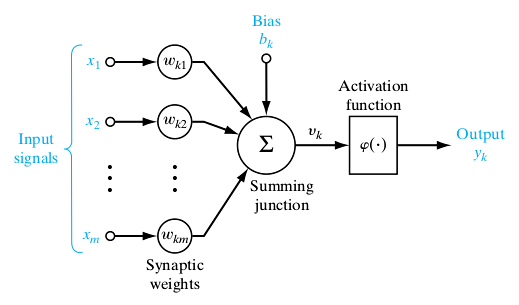
\includegraphics[resolution=100]{Neuron.png}
		\caption{Prosta reprezentacja neuronu.}
\end{figure}


\section{Co to jest sieć neuronowa?}
Koncepcja sztucznej sieci neuronowej to połączenie wielu neuronów w jeden obiekt. Pozwala to na rozpoznawanie bardziej skomplikowanych wzorców i większej różnorodności typów obiektów niż klasyfikacja binarna. Zwykła sieć neuronowa składa się z trzech warstw węzłów. Warstwa pierwsza stanowi warstwę wejściową sieci i składa się z sygnału wejściowego.
Kolejna warstwa jest nazywana warstwą ukrytą, użytkownik nie ma dostępu do niej, przypomina czarną skrzynkę. Nie można zaobserwować co się wewnątrz niej dzieje, użytkownik widzi jakie są dane wejściowe, wartości które powinny zostać zwrócone (w ostatniej warstwie), ale nie ma informacji co jest i powinno się znajdować w tej warstwie podczas trenowania sieci.
Ostatnia warstwa, pojedynczy węzeł nazywany jest warstwą wyjściową. Pobiera wektor wartości wyjściowych z poprzedniej warstwy (ukrytej) i na nim zostaje obliczona wartość wyjściowa (odpowiedź).
Taka architektura nazywa sie siecią dwuwarstwową. Dane wejściowe, mimo że tworzą pierwszą warstwę nie są liczone w nazewnictwie.
Z warstwami ukrytą i wyjściową powiązane są parametry w (ang. weight) oraz b (bias), oznaczające kolejno: macierz wag oraz wektor progów.


\begin{figure}[h]
	\centering
			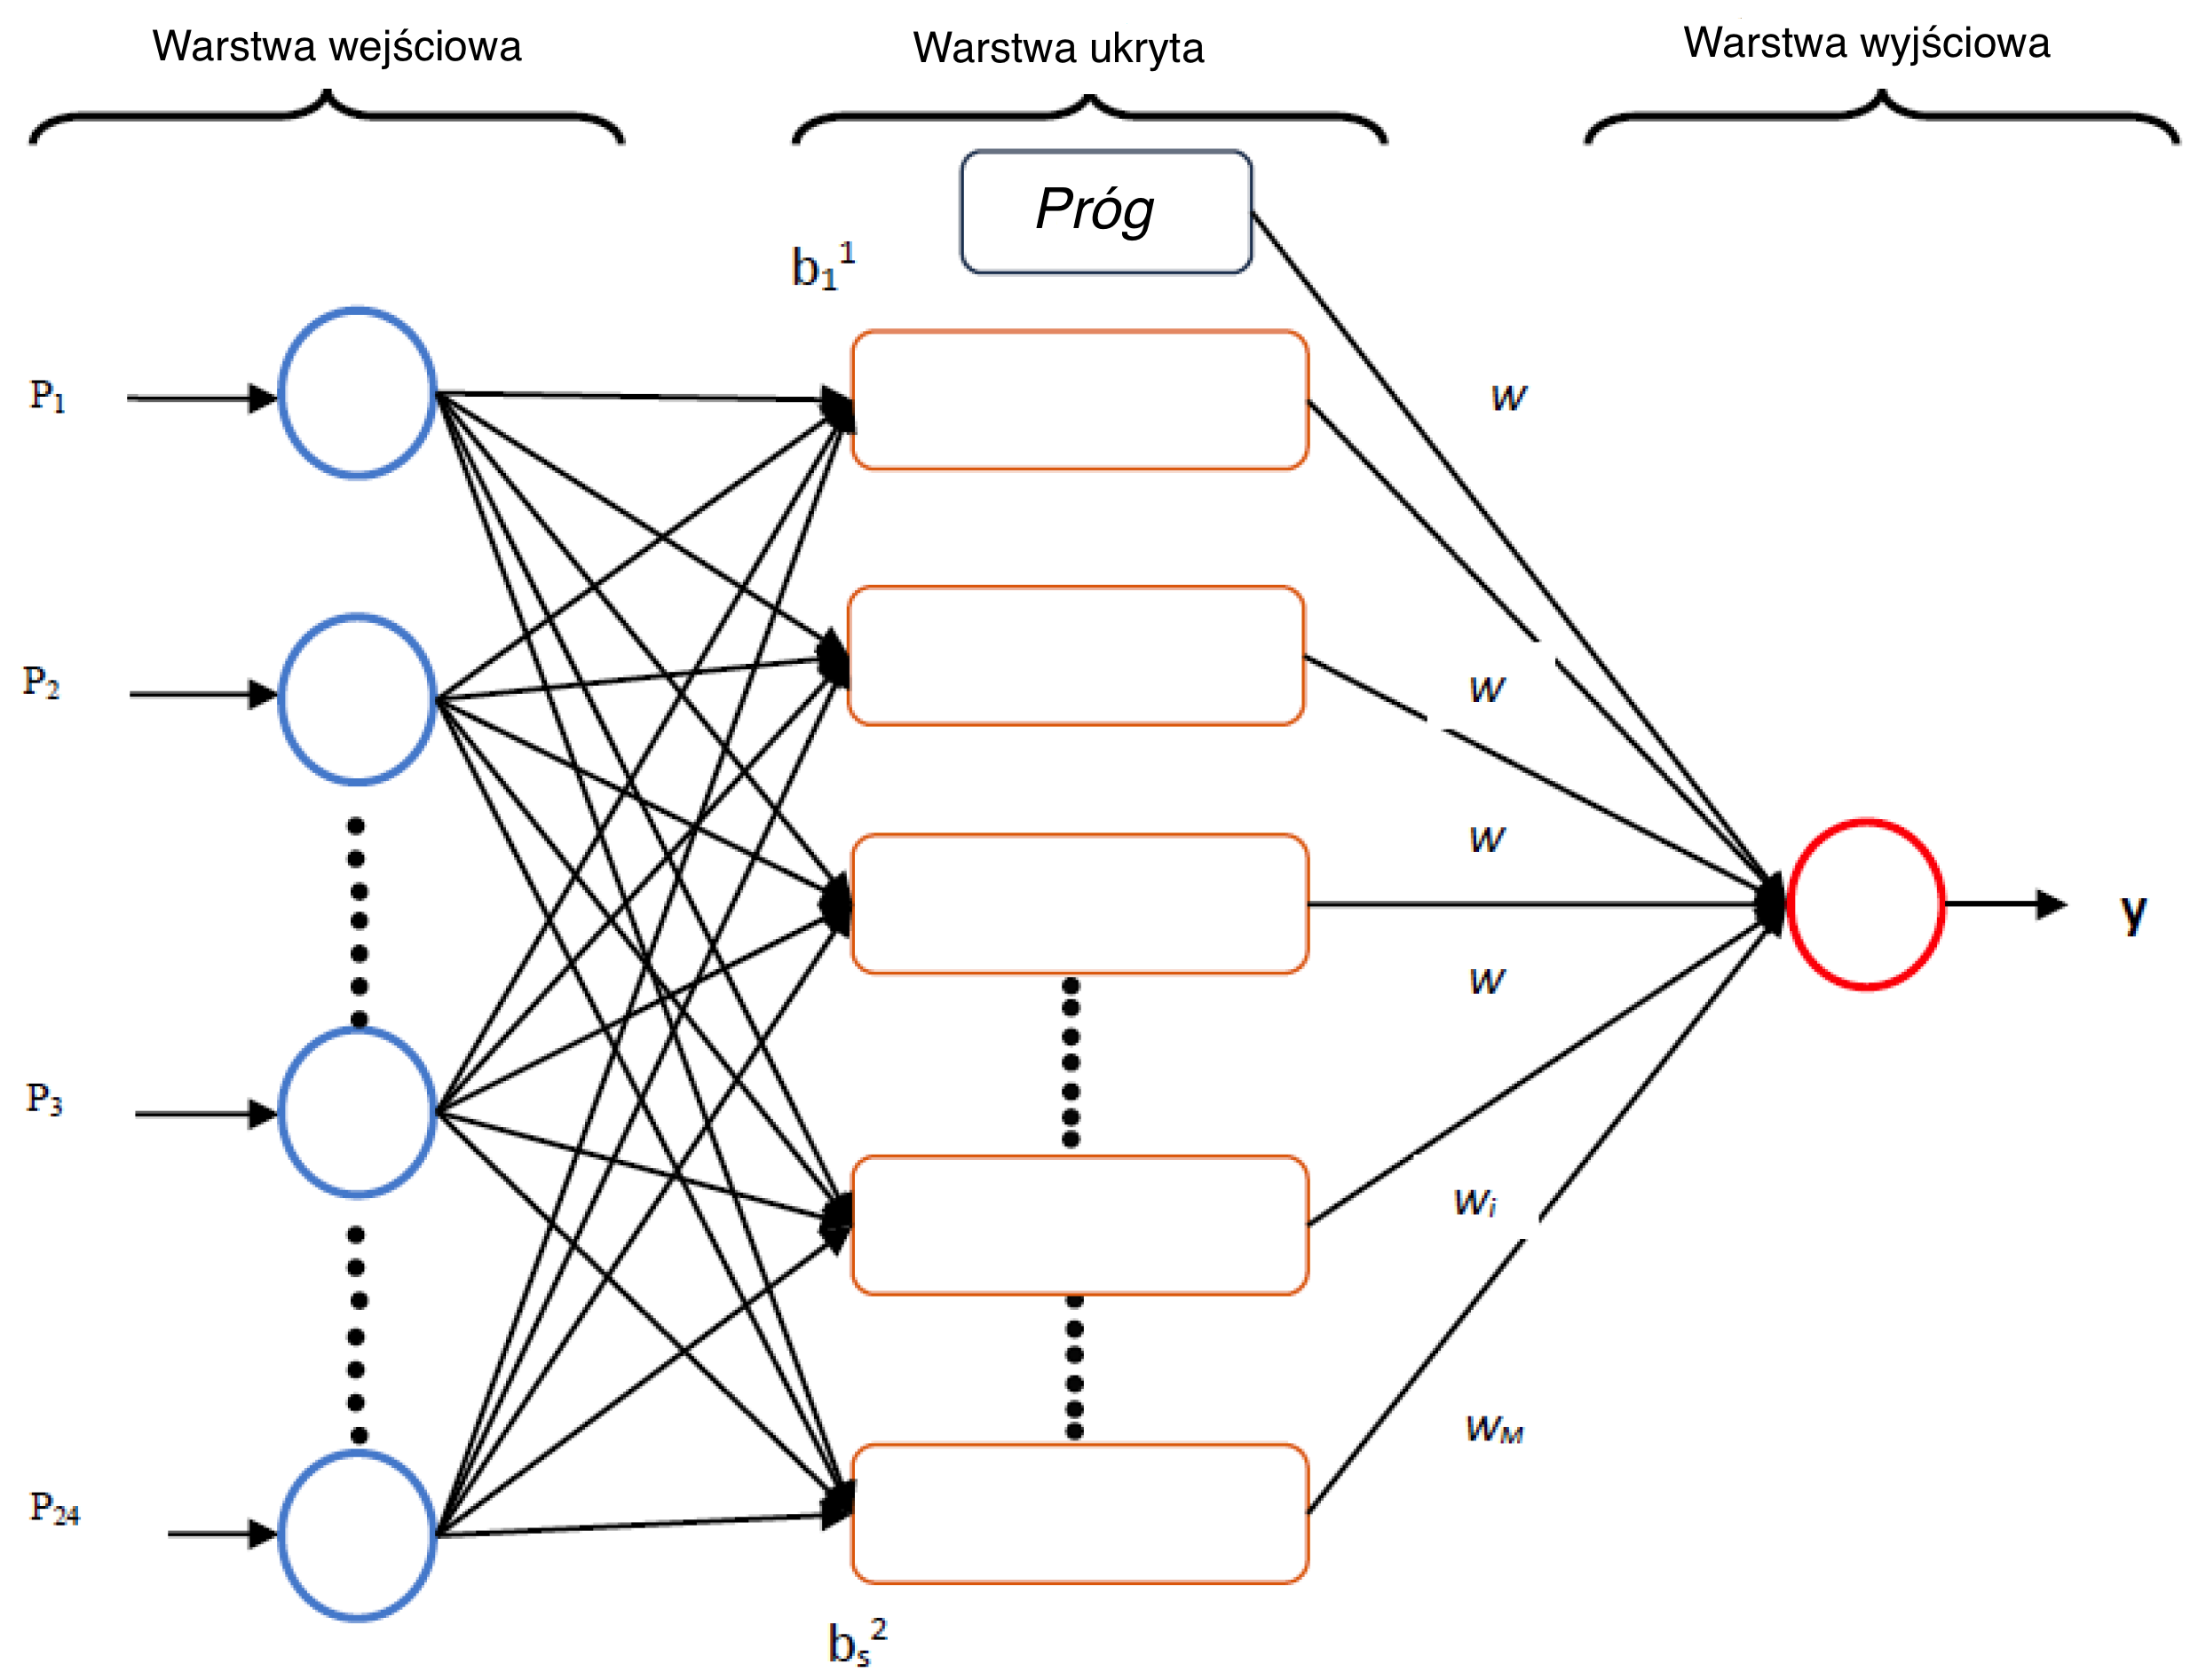
\includegraphics[resolution=100]{SiecNeuronowa.png}
		\caption{Prosta sieć neuronowa złożona z dwóch warstw.}
\end{figure}

\section{Jak uczyć sieci neuronowe}
W obecnym momencie istnieją dwie możliwości by sieć posiadła umiejętność poprawnej klasyfikacji. 

\subsection*{Uczenie nadzorowane}
Jest to typ uczenia maszynowego, które zakłada obecność ludzkiego nauczyciela. Nauczyciel zobowiązany jest stworzyć odpowiednie dane uczące. Takie dane są parą danych, wejściowego obiektu uczącego oraz prawidłową odpowiedź wyjściową do tej danej. System na podstawie tych danych ma nauczyć się przewidywać poprawną odpowiedź dla nowych danych, ze znanej mu domeny.
Zadania uczenie nadzorowanego dzielą się na dwie kategorie, regresję i klasyfikację. W problemie regresji próbuje się przewidzieć wyniki, które są wartościami ciągłymi, czyli mając jakieś dane próbuje się je mapować na funkcję ciągłą. W problemie klasyfikacji algorytm ma za zadanie przewidzieć wyniki będące wartościami dyskretnymi, uściślając jest to znajdowanie klas obiektów, na podstawie danych wejściowych.
Uczenie nadzorowane ma wiele zastosowań, do głównych należą (wraz z używanym typem sieci):
- przewidywanie cen nieruchomości (zwykła sieć neuronowa),
- reklamy internetowe (zwykła sieć neuronowa),
- rozpoznawanie mowy (rekurencyjna sieć neuronowa),
- tłumaczenie maszynowe w translatorach (rekurencyjna sieć neuronowa),
- samochody autonomiczne (sieci hybrydowe lub inne niestandardowe sieci),
- rozpoznawanie obiektów na obrazach (konwolucyjna sieć neuronowa).
Ostatnie z wyżej wymienionych zastosowań jest tematem badanym w tej pracy.

Uczenie nadzorowane dzieli się również binarnie ze względu na strukturę dostarczonych danych. Pierwszy rodzaj danych, dane zawierające konkretną strukturę, zazwyczaj tabela, są bardzo dobrze obsługiwane przez większość znanych wcześniej algorytmów uczenia maszynowego i nie wymagają ogromnej mocy obliczeniowej. Choć sieci neuronowe świetnie się sprawdzają przy tego typu danych, używanie ich ma sens dopiero gdy danych jest bardzo dużo (wielkość tabel przekraczające miliony rekordów). Drugi typ danych, nieustrukturyzowane zdjęcia, pliki audio, tekst, jest znacznie trudniejszy do rozpoznania przez komputer, za to dużo bardziej naturalny dla ludzi. Dzięki głębokim sieciom neuronowym i wielkiej mocy obliczeniowej komputerów, dokładność algorymtów uczących się na tego typu danych znacząco wzrosła, z 70\% do ok 95-99\% dokładności zależnie od ilości danych.

\subsection*{Uczenie nienadzorowane}


\section{Elementy sieci neuronowych} 

\subsection{Metoda gradientu prostego}
Algorytm stosowany do szukania minimum lokalnego płaszczyzny wyznaczonej funkcją. Jest to bardzo prosta metoda optymalizacji stosowana do 
\subsection{Funkcje aktywacji}
\subsection{Wykres obliczeniowy}
\subsection{Propagacja i wsteczna propagacja błędu}


\subsection{Parametry}
Najważniejszy element sieci neuronowej. Składa się na niego zbiór wag i progów (bias). Wagi wyznaczają sposób działania sieci, która ma nauczyć się dobrać odpowiednie parametry przy pomocy algorytmu uczącego, odpowiednio dobranych hiperparametrów oraz zbioru danych uczących. Wagi muszą być dobrane w sposób umożliwiający neuronom wykonanie czynności, których sie od nich wymaga. Ze względu na ilość wag w głębokich sieciach, gdzie dla każdego z tysięcy neuronów może istnieć kilkaset wejść, proces musi być automatyczny. Sieć musi wiedzieć kiedy każdy z neuronów zwiększa swoją dokładność czy nie. Wagi i progi powinny być elastyczne i zmieniać się bardo szybko na początku procesu uczenia i tylko w niewielkim stopniu zmieniać wartości kiedy algorytm kończy proces uczenia.

\subsection{Hiperparametry}
Tworzenie dobrej sieci neuronowej wymaga nie tylko parametrów ale również dobrego doboru hiperparametrów. Elementy "ręcznie" dobierane dla algorytmu uczenia. Najczęściej ustawiane parametry dla sieci neuronowej to:
- stała uczenia,
- ilość iteracji uczenia w jednej epoce,
- ilość ukrytych warst,
- ilość ukrytych jednostek,
- wybór funkcji aktywacji (ReLU, tangens, sigmoida),
- parametry regularyzacji,
- rozmiary próbek uczących,
i wiele innych mniej ważnych hiperparametrów
Są to parametry kontrolujące sposób wykonania algorytmu uczącego i w ostateczności to one mają największy wpływ na zwykłe parametry wagi i progi (bias). Nie został ustalony jednolity sposób doboru hiperparametrów. Zwyczajowo stosuje się metodę prób i błędów na podstawie tego jak algorytm się zachowuje.\cite{deeplearningAI} Za każdą zmianą wartości należy uruchomić algorytm i sprawdzić jak zachowuje się funkcja kosztu, jeśli maleje lepiej niż przy porpzednich wartościach można stroić dalej w tym kierunku. Dopieranie odpowiednich wartości niestety jest procesem empirycznym i należy wyrobić odpowiednią intuicję aby jak najtrafniej dobierać parametry od początku. Wartości te też nie są stałe, zmieniają się w zależności od dziedziny badanego zagadnienia. Być może najbliższe lata przyniosą dobry i spójny przewodnik dobierania najlepszych wartości, pozwoli to znacznie zautomatyzować proces.

\subsection{Jak zbudować sieć neuronową}

% ################################
%        DEEP LEARNING
% ################################

\chapter{Deep Learning}
%Rozdział opisujący różnicę między deep learningiem a zwykłymi sieciami. Osiągnięcia związane z Deep Learningiem i boom na AI.
\section{Techniki tworzenia głębokich sieci}
W tym rozdzial zostają przybliżone trzy interesujące techniki głębokiego uczenia. Zostały wybrane ze względu na ich obszerną ilość zastosowań oraz potencjał, który można wykorzystać przy rozpoznawaniu wzorców na obrazach. Następnie opiszę kilka bibliotek implementujących wsparcie dla większości architektur sieci przedstawionych w pracy. Biblioteki są wybrane na podstawie przekroju platform i języków mi znanych. 

\subsection{Sieci neuronowe}
\subsection{Convolutional Neural Networks}
Inaczej znane jako
\subsection{Recurrent Neural Networks}
\subsection{Fully Convolutional Networks}

\chapter{Biblioteki implementujące uczenie głębokich sieci neuronowych}

\subsection{Tensorflow}
\begin{figure}[h]
	\centering
			
\includegraphics[resolution=120]{Tensorflow.png}
		\caption{Logo biblioteki Tensorflow}
\end{figure}
Pierwsza otwarta biblioteka od Google. Obecnie najczęściej używana podczas prac naukowych, o czym świadczy ilość cytowań[1]. Od 2018 roku dostępna również pod nazwą Tensorflow.js jako biblioteka javascript, udostępniające ten sam interfejs programistyczny.

\subsection{Keras}
\begin{figure}[h]
	\centering
			
\includegraphics[resolution=120]{Keras.png}
		\caption{Logo biblioteki Keras}
\end{figure}
Keras jest frameworkiem udostępniającym wysokopoziomowe API sieci neuronowych. Działanie opiera się na wykorzystaniu Tensorflow, CNTK lub Theano jako bibliotek wykonujących obliczenia. Głównym założeniem tego oprogramowania jest możliwość szybkiego wykonywania eksperymentów, co ma się przełożyć na lepsze badanie uczenia maszynowego.

\subsection{PyTorch}
\begin{figure}[h]
	\centering
			
\includegraphics[resolution=120]{PyTorch.png}
		\caption{Logo biblioteki PyTorch}
\end{figure}

\subsection{Tensorflow.js [Deeplearn.js]}
\begin{figure}[h]
	\centering
			
\includegraphics[resolution=120]{TensorflowJS.png}
		\caption{Logo biblioteki Tensorflow.js}
\end{figure}
Znany dawniej jako DeepLearning.js Pierwszy zestaw uczenia maszynowego do użycia w przeglądarce. Działa w oparciu o WebGL. Dostarcza calej mocy Tensorflow do przeglądarki czy dowolnego interpretera kodu Javascript.

\subsection{PaddlePaddle}
\begin{figure}[h]
	\centering
			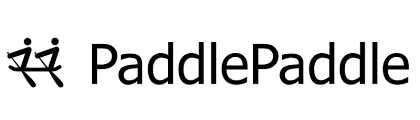
\includegraphics[resolution=120]{PaddlePaddle.png}
		\caption{Logo biblioteki Paddle}
\end{figure}
Chińskie oprogramowanie, mało znane w Europie / USA, za to jest to najpopularniejszy framework w Chinach. Uważam że zasługuje na wyróżnienie ze względu na unikalny charakter. Paddle jest open-source, jednak większość dokumentacji jest w języku kantońskim.

\subsection{MXNet}
\begin{figure}[h]
	\centering
			
\includegraphics[resolution=120]{MXNet.png}
		\caption{Logo biblioteki MXNet}
\end{figure}

\subsection{Caffe2}
\begin{figure}[h]
	\centering
			
\includegraphics[resolution=120]{Caffe2.png}
		\caption{Logo biblioteki Caffe2}
\end{figure}

\subsection{ML.NET}
\begin{figure}[h]
	\centering
			
\includegraphics[resolution=120]{ML_NET.png}
		\caption{Logo biblioteki ML.NET}
\end{figure}
Nowe oprogramowanie od Microsoftu, udostępnione na licencji [licencja], głównie polecane programistom w środowisku .NET. Docelowo ma stać się częścią .NET Core. Nastawione na łatwość integracji z oprogramowaniem biznesowym, chmurą Azure oraz łatwość obsługi przez programistów pracujących w technologiach Microsoftu.

\subsection{PyBrain}
\begin{figure}[h]
	\centering
			
\includegraphics[resolution=120]{PyBrain.png}
		\caption{Logo biblioteki PyBrain}
\end{figure}


\subsection{CNTK}
[Microsoft Research, 2016] - nazwa kompletna Microsoft Cognitive Toolkit. Jest to zestaw narzędzi z działu badawczego Microsoftu, zajmującego sie Deep Learningiem. Narzędzie opisuje sieci neuronowe jako szereg obliczeń na grafie skierowanym. W tym grafie węzły (liście) reprezentują wartości wejściowe oraz parametry sieci, zaś pozostałe węzły są operacjami macierzowymi na ich wejściu. Cognitive Toolkit pozwala użytkownikom w prosty sposób tworzyć i łączyć popularne modele jak (ang. fast-forward Deep Neural Networks), konwolucyjne sieci neuronowe, rekurencyjne sieci neuronowe. Implementuje algorytm spadku gradientowego, wsteczną propagację błędów z automatycznym skalowaniem na wiele urządzeń GPU rozproszonych na różnych serwerach.
CNTK działa na systemach operacyjnych Windows i GNU\\Linux.
\begin{figure}[h]
	\centering
			
\includegraphics[resolution=120]{CNTK.png}
		\caption{Architektura sieci CNTK}
\end{figure}

% ################################
%        ARCHITEKTURA
% ################################

\chapter{Architektura}
\section{Znaczenie architektury dla wydajności sieci}
Sieci neuronowe można ułożyć na nieskończenie wiele sposobów. Aby uzyskać dobre rezultaty należy sprawdzić kilka architektur i jak się zachowują dla dla posiadanych zbiorów danych i zadanych hiperparametrów.
W zależności od typu architektury sieci można osiągnąć zupełnie inne wyniki uczenia dla tych samych algorytmów. 
Architektury różnią się właściwie wszystkim, ilością warstw ukrytych ilością neuronów w warstwie ukrytej. 
Poglądy Tadeusiewicza na architekturę sieci neuronowych.

“Właśnie taka (warstwowa) struktura sieci wyjątkowo łatwo i wygodnie da się wytwarzać zarówno w formie modelu elektronicznego, jak i da się symulować w formie programu komputerowego. Dlatego badacze przyjęli właśnie strukturę warstwową i od tej pory stosują ją we wszystkich sztucznych sieciach neuronowych. Z pełną wiernością biologicznemu oryginałowi ma to niewiele wspólnego, ale jest praktyczne i wygodne. W związku z tym wszyscy tak postępują, nie martwiąc się ani przesłankami biologicznymi, ani dowodami wskazującymi, że architektura sieci bardziej wymyślnie dostosowanej do charakteru zadania może znacznie lepiej realizować stawiane zadania.”

Tak napisał w 2007 roku, kiedy architektury sieci nie miały miały większego znaczenia ponieważ większość sieci była stosunkowo płytka (do 5 warstw ukrytych). Zbiory na których pracowano były stosunkowo niewielkie w porównaniu z dzisiejszymi zasobami skatalogowanych obrazów. 
Obecnie istnieją dowody (choćby coroczne zawody ImageNet, w których udowadnia się że struktura sieci ma znaczenie. Może poprawić szybkość i dokładność uczenia). Profesor jest ekspertem w dziedzinie sieci neuronowych, jednak jego książki i poglądy są z lat 1990 - 2010. Późniejsze jego prace są dużo mniej znane.

\section{Przegląd najbardziej efektywnych architektur}

\subsection{AlexNet}
 [Alex Krizhevsky, Ilya Sutskever, Geoffrey E. Hinton, 2012] - pierwsza prawdziwa konwolucyjna sieć neuronowa (CNN), która pomogła zmienić opinię na temat uczenia głębokiego. Została zaimplementowana z użyciem biblioteki CUDA. Pierwsza sieć neuronowa, ucząca się z powodzeniem dla dużego zbioru danych.
 Została wytrenowana na zbiorze danych złożonym z ponad 15 milionów obrazów podzielonych na 22000 klas. 
 W testach top-1 i top-5 uzyskała wartości kolejno 37,5\% i 17\%, co pozwoliło wygrać konkurs ImageNet Large Scale Visual Recognition Challenge. 
 Sieć neuronowa zawiera 60 milionów parametrów i 650 000 neuronów. Architekturę tworzy 8 warstw, gdzie pierwsze 5 to warstwy konwolucyjne, a pozostałe 3 są warstwami w pełni połączonymi, ta ostatnia ma oczywiście 1000 wyjść z funkcji softmax. AlexNet znacząco przewyższyła swoją wydajnością poprzednich uczestników i wygrała zawody redukując błąd top-5 do 15,32\%. Drugie miejsce to błąd ok 26.2\% (nie była to CNN). Sieć jest głęboką modyfikacją architektury Yann’a LeCunn’a. AlexNet była zaplanowana na dwie karty graficzne, stąd rozdzielenie przepływu informacji na 2 części. Trenowanie sieci na 2 GPU było nowością na te czasy. Sieć została wytrenowana na zbiorze ImageNet. Do wyliczenia funkcji nieliniowych były używane ReLU (tutaj po raz pierwszy okazało się że ReLU działa dużo szybciej niż tanh). Sieć o której będą uczyły się dzieci na lekcjach historii. \cite{NIPS2012_4824}

\begin{figure}[h]
	\centering
			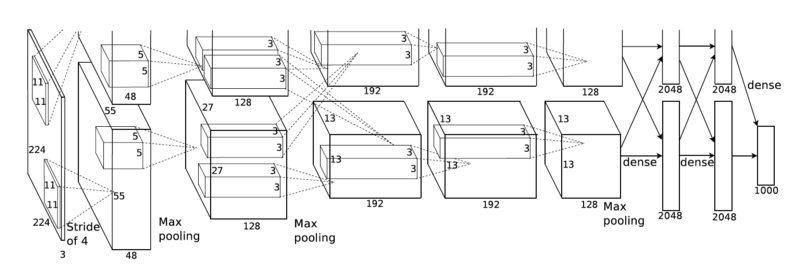
\includegraphics[resolution=120]{AlexNet.png}
		\caption{Architektura sieci AlexNet}
\end{figure}

\subsection{LeNet}
[Authors, Year] - Jest to obecnie mało znacząca architektura. Pierwsze praktyczne zastosowanie sieci konwolucyjnych jeszcze w latach 90’tych. Używana była do prostych zadań: czytanie kodów pocztowych, liczb.\cite{Lecun98gradient-basedlearning}

\begin{figure}[h]
	\centering
			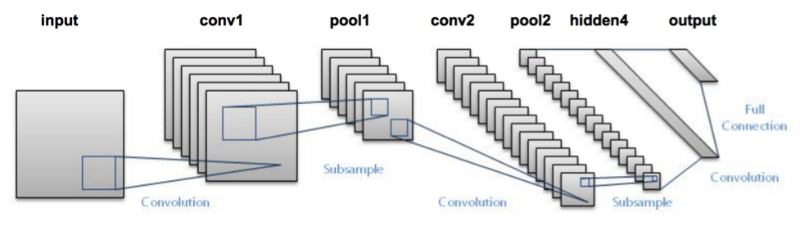
\includegraphics[resolution=120]{LeNet.png}
		\caption{Architektura sieci LeNet}
\end{figure}

\subsection{VGG Net}
 [Simoyan i Zisserman, 2014] - sieć złożona z 16 warstw konwolucyjnych, która charakteryzuje się małymi filtrami i duża głębokość sieci.
W trakcie trenowania sieci wyjście jest ustawione na ustalony rozmiar (224 x 224 x 3). Przetwarzanie wstępne obejmuje odjęcie mediany wartości RGB dla każdego piksela. Zdjęcie jest przetwarzanie przez stos warstw konwolucyjnych, gdzie używane są filtry o bardzo małym polu widzenia (3x3) [najmniejszy możliwy rozmiar by móc rozpoznać kierunek]. Operacja Max-pooling jest wykonana na polu 4 pikseli, co pokazuje że jest to pobieranie jak najmniejszych cech z obrazu. Ukryte warstwy są wyposażone w nieliniową funkcję aktywacji ReLU. Po stosie warstw konwolucyjnych, następuje nałożenie 3 warstw w pełni połączonych (to takie duże warstwy zawierające wszystkie cechy?). Pierwsze dwie mają 4096 kanałów, trzecia już tylko 1000 (po jednym kanale na klasę obiektu). Obecnie architektura ta jest dość popularnym wyborem dla wyodrębniania cech ze zdjęć. Konfiguracje wag dla zbioru obrazów z ImageNet są dostępne online. W tej sieci problemem jest 140 milionów parametrów, którymi czasem trzeba zarządzać. \cite{DBLP:journals/corr/SimonyanZ14a}

\subsection{GoogleNet / Inception}
[Christian Szegedy, Wei Liu, Yangqing Jia, Pierre Sermanet, Scott Reed, Dragomir Anguelov, Dumitru Erhan, Vincent Vanhoucke, Andrew Rabinovich, 2014] - produkt jak nazwa wskazuje wyszedł z firmy Google. Charakteryzuje się przełomową poprawą użycia zasobów wewnętrznych. ImageNet jest zaprojektowana na jak największą szerokość i głębokość jednocześnie utrzymując stałe zużycie mocy obliczeniowej. Optymalizacja jakości opiera się na zasadzie Hebbian’a (jest to teoria neuronauki, która mówi o adaptacji neuronów w trakcie nauki). Błędy klasyfikacji wynoszą top-1: 17,2\% i top-5: 3,58\% (dla v3). Sieć składa się łącznie z 22 warstw. Sieć jest modułowa, gdzie każdy moduł pełni rolę wielopoziomowego ekstraktora cech przeliczającego konwolucje na macierzach rozmiarów 1x1, 3x3, 5x5. Zaletą tej architektury są bardzo małe rozmiary wag (mniej niż 100MB dla v3). Kolejną ważną zaletą jest ilość parametrów, tylko 4 miliony co jest wynikiem 12 razy lepszym od AlexNet. Jest to jedna z najbardziej złożonych sieci względem architektury modułowej. W wersji naiwnej każda warstwa posiada 4 ekstraktory cech (3 konwolucyjne i jedną 3x3 max pooling), następnie wartości te są składane i wysyłane do warstwy wyżej. Do poprawienia wydajności obliczeniowej pozbyto się warstwy “w pełni połączonej”. \cite{DBLP:journals/corr/SzegedyLJSRAEVR14}

\subsection{ResNet}
[Kaiming He et al, 2015]  - architektura oparta na mikro modułach. Charakteryzuje się możliwością odrzucania połączeń i posiada ogromny moduł na normalizację zbioru iteracji (batch normalization). Normalizacja jest pomysłem zaczerpniętym z rekurencyjnych sieci neuronowych. Ta technika pozwala stworzyć sieć ze 152 warstwami ukrytymi przy zachowaniu złożoności mniejszej niż VGG. \cite{DBLP:journals/corr/XieGDTH16}
\begin{figure}[h]
	\centering
			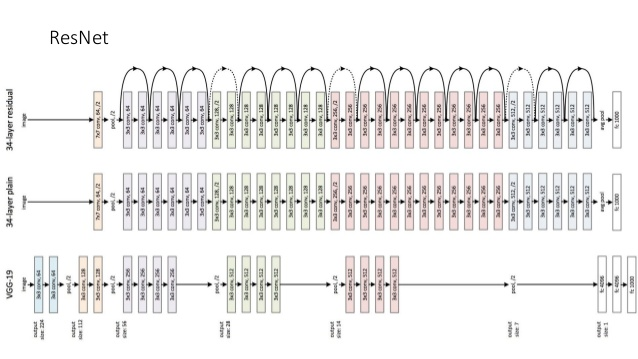
\includegraphics[resolution=120]{ResNet.png}
		\caption{Architektura sieci ResNet}
\end{figure}

\subsection{ResNeXt}
[Saining Xie, Ross Girshick, Piotr Dollar Zhuowen Tu Kaiming He, 2017] - modularyzowalna 
\cite{DBLP:journals/corr/XieGDTH16}
\begin{figure}[h]
	\centering
			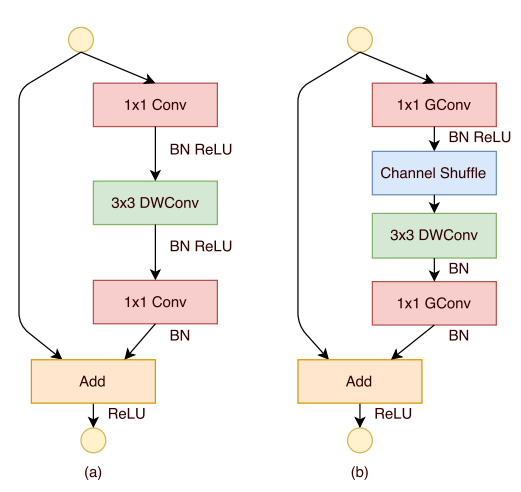
\includegraphics[resolution=120]{ResNeXt.png}
		\caption{Architektura sieci ResNeXt}
\end{figure}

\subsection{RCNN -- obrazek jest zastępczy nie ma nic w internecie interesującego}
[Authors, Year] - \cite{DBLP:journals/corr/RenHG015}
\begin{figure}[h]
	\centering
			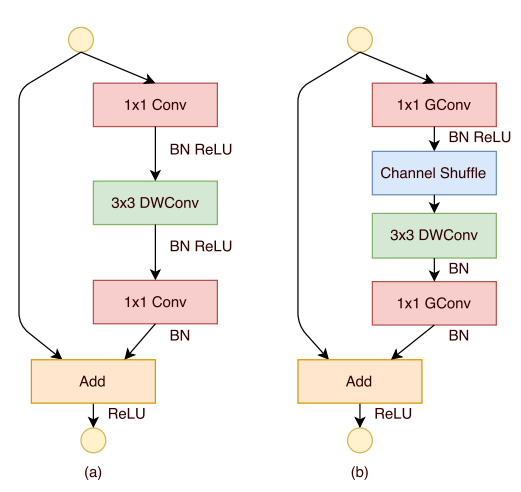
\includegraphics[resolution=120]{ResNeXt.png}
		\caption{Architektura sieci RCNN}
\end{figure}

\subsection{YOLO - You Only Look Once }
[Joseph Redmon, Santosh Divvala, Ross Girshick, Ali Farhadi, 2016] - You Only Look Once jest systemem wykrywania obiektów w czasie rzeczywistym. Obraz jest dzielony na części oddzielonymi od sieibie prostokątami, ..???
Cały przepływ danych do wykrycia obiektów jest jedną siecią, dlatego może być zoptymalizowany \cite{DBLP:journals/corr/RedmonDGF15}
\begin{figure}[h]
	\centering
			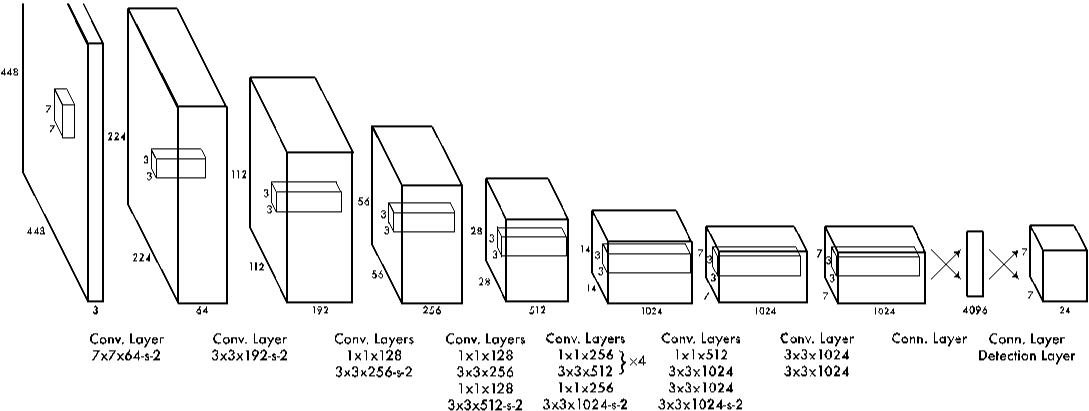
\includegraphics[resolution=120]{YOLO.png}
		\caption{Architektura sieci YOLO}
\end{figure}

\subsection{SqueezeNet}
[Authors, Year] - \cite{DBLP:journals/corr/IandolaMAHDK16}
\begin{figure}[h]
	\centering
			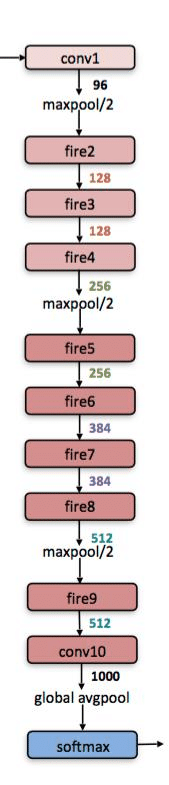
\includegraphics[resolution=120]{SqueezeNet.png}
		\caption{Architektura sieci SqueezeNet}
\end{figure}

\subsection{SegNet}
[Authors, Year] - \cite{DBLP:journals/corr/BadrinarayananH15}
\begin{figure}[h]
	\centering
			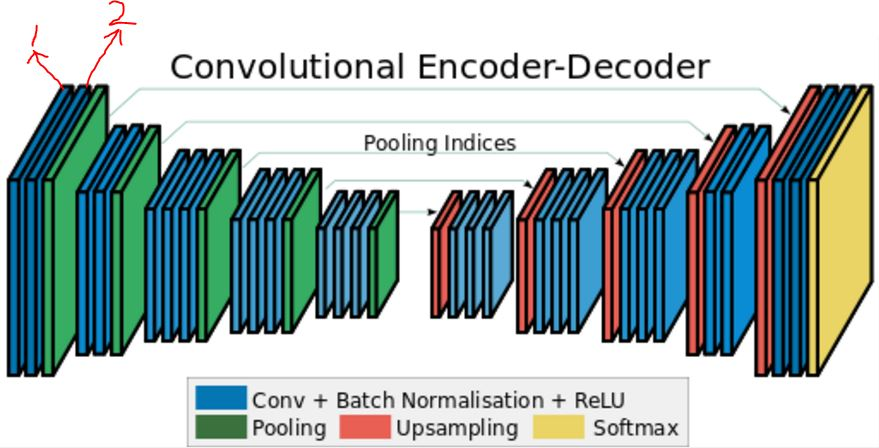
\includegraphics[resolution=120]{SegNet.png}
		\caption{Architektura sieci SegNet}
\end{figure}

\subsection{Generative Adversarial Network}
[Ian J. Goodfellow, Jean Pouget-Abadie, Mehdi Mirza, Bing Xu, David Warde-Farley, Sherjil Ozair†, Aaron Courville, Yoshua Bengio‡, 2014] - w skrócie GAN. Są architekturą sieci neuronowych skomponowanych z dwóch sieci przeciwstawionych wobec siebie. Zaprojektowane na uniwersytecie w Montrealu (gdzie powstało większość przełomów dotyczących neuronów) przez największe obecnie autorytety w dziedzinie. GAN obudził duze nadzieje na szybkie i "twórcze" działania algorytmów, jego najczęstszym zastosowaniem jest tworzenie komputerowych "dzieł sztuki". Jak to działa? Jedna sieć generuje kandydatów, a druga ich ocenia wytworzone obiekty. W ten sposób obie sieci uczą się od siebie wzajemnie. - \cite{NIPS2014_5423}
\begin{figure}[h]
	\centering
			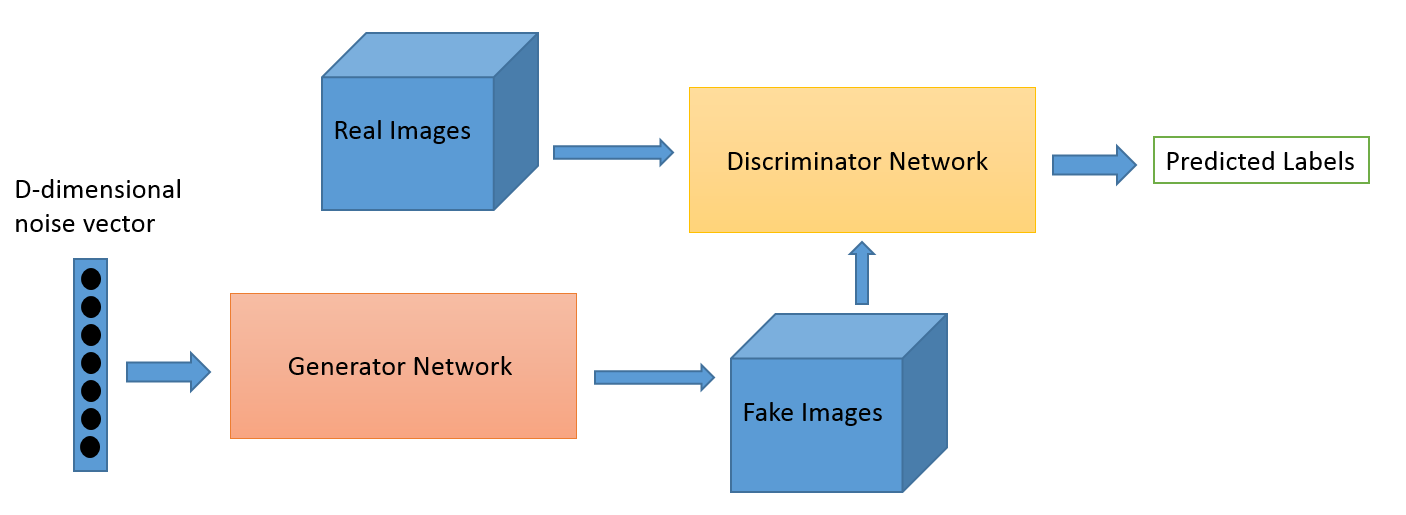
\includegraphics[resolution=120]{GAN.png}
		\caption{Architektura sieci GAN}
\end{figure}


% ################################
%        PORÓWNANIE WYDAJNOŚCI ARCHITEKTUR
% ################################
\chapter{Testy wydajności}

% ################################
%        PODSUMOWANIE
% ################################

\chapter{Podsumowanie} 

% ################################
%        SPIS RYSUNKÓW
% ################################

\addcontentsline{toc}{chapter}{Spis rysunków}
\listoffigures

% ################################
%        BIBLIOGRAFIA
% ################################
\bibliographystyle{plain}
\bibliography{bibliography/alexnetNips,bibliography/deeplearningbook,bibliography/dropout,bibliography/fastAI,bibliography/ganArxiv,bibliography/googleNet,bibliography/lecun,bibliography/medicalImage,bibliography/microsoftResNet,bibliography/rCNN,bibliography/relu,bibliography/resnextArxiv,bibliography/VGGNet,bibliography/ZFNet,bibliography/ResNeXt,bibliography/YOLO,bibliography/SqueezeNet,bibliography/SegNet} 

\end{document}